% SPDX-License-Identifier: CC-BY-SA-4.0
% Author: Matthieu Perrin
% Part: 
% Section: 
% Sub-section: 
% Frame: 

\begingroup

\begin{frame}{Sémaphore}
  \begin{center}
    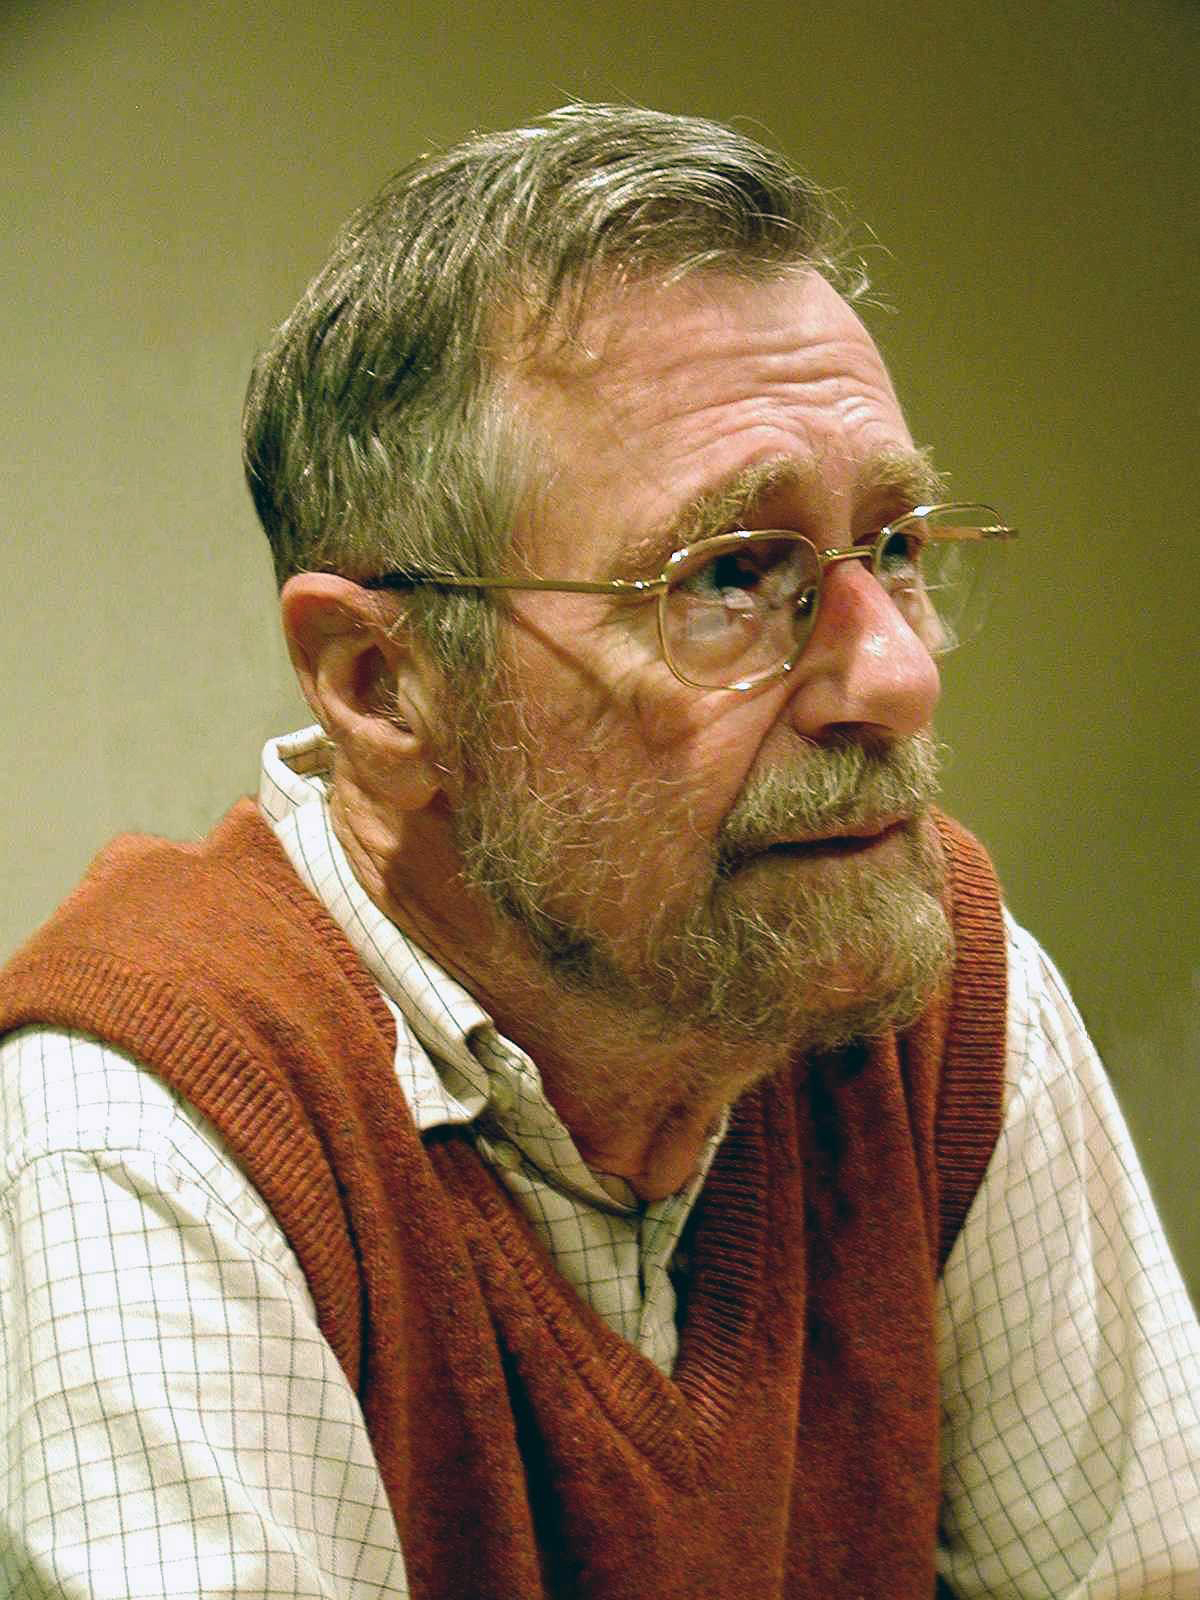
\includegraphics[height=2cm]{Dijkstra}\\
    Edsger W. Dijkstra
  \end{center}
  \vFill
  \begin{block}{Classe \lstinline{java.util.concurrent.Semaphore}}
      \begin{itemize}
      \item \lstinline{new Semaphore(n)}
	\begin{enumerate}
	\item Initialise un sémaphore avec $n$ jetons
	\end{enumerate}
      \item \lstinline{public void acquire() throws InterruptedException}
	\begin{enumerate}
	\item S'il reste un jeton, donner un jeton.
	\item Sinon, attendre qu'un jeton se libère.
	\end{enumerate}
      \item \lstinline{public void release()}
	\begin{enumerate}
	\item Libérer un jeton.
	\end{enumerate}
      \end{itemize}
  \end{block}
  \vFill
  \begin{citing}
  \item[D62] Edsger W. Dijkstra. \textit{Over de sequentialiteit van procesbeschrijvingen (About the sequentiality of process descriptions)} (1962-1963)
  \end{citing}
\end{frame}

\endgroup
\endinput
